\documentclass[fleqn, 10pt]{article}

% Paquetes necesarios
\usepackage[utf8]{inputenc}
\usepackage[english]{babel}
\usepackage{amsthm, amsmath}
\usepackage{nccmath} %Para centrar ecuaciones
\usepackage{graphicx}
\graphicspath{ {Documentos/} }
\usepackage{tikz}
\usepackage{amssymb}
\usepackage[linesnumbered]{whilecode2}

% Personalizo mi alfabeto
\DeclareMathAlphabet{\pazocal}{OMS}{zplm}{m}{n}
\newcommand{\Lb}{\pazocal{L}}

% Definimos los entornos para definiciones, teoremas, etc...
\theoremstyle{plain}
\newtheorem{proposicion}{Proposición}

\theoremstyle{definition}
\newtheorem{definition}{Definición}[section]
\newtheorem{example}{Ejemplo}[section]

%Definimos el título
\title{Teoría de Autómatas y Lenguajes Formales\\[.4\baselineskip]Práctica 4}
\author{Irene, Recio López}
\date{\today}

%Comienzo del documento
\begin{document}

%Generamos el título
\maketitle

\subsubsection*{Ejercicio 1: El desarrollo del cálculo de la menor codificación del programa WHILE "diverger"}

\whileprogram{Q}{0,2}{}{S}
\begin{whilecode}[H]
	$X_2 \Assig X_1 + 1$\;
 	\While{$X_2 \not = 0$}{
  	$X_1 \Assig 0$\;
	}
\end{whilecode}


\subsubsection*{Ejercicio 2: El código Octave que hace  un print de todos los vectores, y una captura de ejemplo de ejecución}

\begin{verbatim}
function printNvectors(N)
  for i=0:N-1
    disp([ ' ( ' num2str(godeldecoding(i)) ' ) ' ])
  end
end
\end{verbatim}

\centering	
	\includegraphics[scale=0.7]{P4ejercicio2}

\newpage
\subsubsection*{Ejercicio 3: El código Octave que hace un print de todos los programas WHILE, y una captura de ejemplo de ejecucion}


\begin{verbatim}
function printNwhilePrograms(N)
  for i=0:N-1
    disp(N2WHILE(i))
  end
 end
\end{verbatim}
\centering
	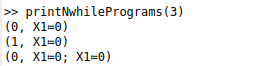
\includegraphics[scale=0.7]{P4ejercicio3}

\end{document}

